\section{Docker image}
\label{sec:intro:docker_image:docker_img}
This section explains the Docker image in more detail. 
First the architecture of a Docker image with the most necessary information for subsequent work is presented. 
Then the construct for building a Docker image is explained. 
Lastly a description of the metadata information of an image takes place. 
These basics are eminentely important because they are part of the theoretical concept.

\subsection{Image architecture}
\label{sec:intro:docker_image:docker_img:architecture}
A Docker image is ultimately a stack of selected file system layers to provide a starting point for a container \cite{docker_images}.
Figure \ref{sec:intro:docker_image:docker_image_stack} shows how a Docker image is stacked. 
The Linux kernel is always at the bottom. A Debian and a Busybox layer are placed on the kernel.
Both already form a complete and runnable Docker image.
On top of these layers more layers can be stacked as shown on the Debian layer with an additional Emacs and an Apache layer. 
The Busybox layer does not have further layer placed on the top.
Docker finally attaches a read/write file system across all underlying layers when a container is launched from an image.
\begin{figure}[htbp]
 \centering
 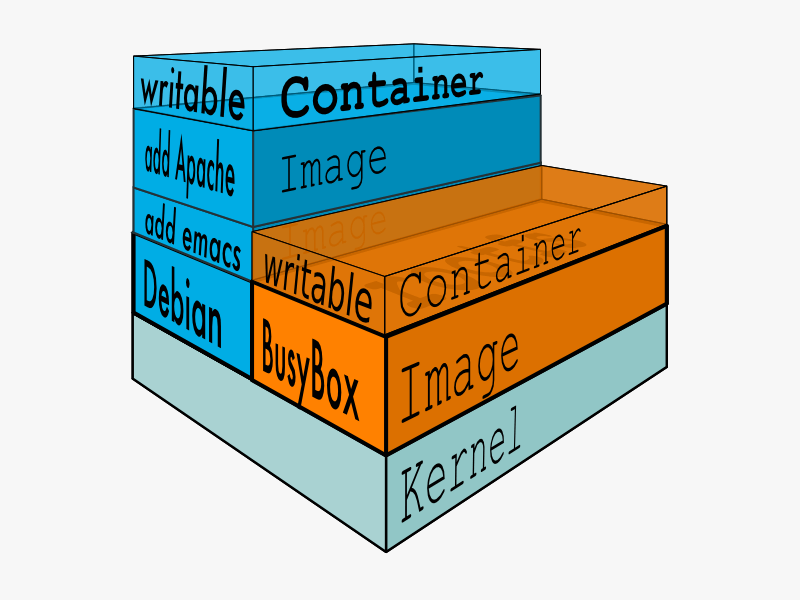
\includegraphics[width=0.6\textwidth]{gfx/examples/docker-filesystems-busyboxrw}
 \caption{Stacked union filesystems represents a Docker image}
\label{sec:intro:docker_image:docker_image_stack}
\end{figure}

Docker uses storage drivers in order to manage images and corresponding file system layers \cite{docker_storage_driver}. 
A storage driver mainly handles the details about the way these layers interact with each other.
There are several storage drivers available like ZFS, BTRFS and many more which can be configured by the responsible system engineer or developer. 
These storage drivers have advantages and disadvantages which should be carefully considered. 
Docker uses in the latest version Overlay2 as storage driver per default \cite{docker_storage_driver}. 
The Overlay2 informations about an image can be viewed by the Docker inspect command.
\begin{lstlisting}
	docker inspect ubuntu
\end{lstlisting}
The inspection only shows the part that is interesting for the Docker image architecture.
\lstinputlisting[caption={Overlay2 informations about Docker image}, firstline=71, lastline=79, captionpos=b, label={sec:intro:docker_image:corresponding_unionfs}]{chapters/intro/listings/inspect_results.txt}
As seen in Listing \ref{sec:intro:docker_image:corresponding_unionfs} the introduced Overlay2 elements and mechanisms are completely used.
This shows once again that Docker only uses the well-known Linux core functions instead of building own mechanisms.

One interesting and important fact exists about the mount process.
The Overlay2 storage driver has a symbolic link for each image layer implemented. 
During the mount process these symbolic links are used instead for the real folder names. 
The reason is the total length of 65 characters for each folder name. 
These symbolic links help avoid the Linux \textit{mount} command from exceeding page size limitation.
It is also important to note that the \textit{diff} directory in each layer builds the chain of the overlay. 
In each layer additional helper files are available like the lowerfile which creates a relation to an associated parent. 
This lowerfile only exists if a parent folder exist. 
The lower files are responsible for creating the chain of lowerdirs which can be seen in Listing \ref{sec:intro:docker_image:corresponding_unionfs}.

Every Docker image has a name and a tag. A special convention is described in \cite{docker_tag} and now explained. 
An image name is made up of slash-separated name components optionally prefixed by a registry hostname. 
The hostname must comply with standard DNS rules but may not contain underscores. 
A tag name must be valid ASCII and may contain lowercase and uppercase letters, digits, underscores, periods and dashes. 
A tag name may not start with a period or a dash and may contain a maximum of 128 characters.
It is important to know that the name and the tag are separated by a colon.
The understanding of the naming and tagging connection is helpful, since it finds application in the following chapters.
In the following the construct of building a Docker image is described.

\subsection{Dockerfile}
\label{sec:intro:docker_image:docker_img:dockerfile}
Docker Inc. introduced a construct called Dockerfile in order to build a Docker image.
Each entry in this Dockerfile starts with a keyword. 
These keywords can be used by a developer to assemble an image. 
Each entry in a Dockerfile creates a different file system layer. 
In other words each file system layer represents an instruction with help of a keyword in a Dockerfile.
The Dockerfile construct provides around 20 keywords \cite{dockerfile_ref}.
Listing \ref{sec:intro:docker_image:dockerfile} shows a typical Dockerfile.
\lstinputlisting[caption={Dockerfile to create a container image}, captionpos=b, label=sec:intro:docker_image:dockerfile]{chapters/intro/listings/dockerfile.txt}
The FROM statement starts out by creating a layer from the ubuntu 18.04 image. 
COPY adds an example bash script from the Docker client’s current directory. 
RUN makes the program executable. 
Finally CMD specifies which command has to be executed inside the container.

An image can be created with the corresponding Dockerfile and the Docker build command. The responsible command is shown below.
\begin{lstlisting}
	docker build <my_new_image> -f <dockerfile>
\end{lstlisting}
The Dockerfile construct is valuable to know because it is responsible for integrating secrets into an image. 
Logically there are two categories that are responsible for integrating static files.
First \textit{direct integration} which is related the actions COPY and ADD. T
he difference between the two commands is the range of functions. 
ADD is contrary to COPY able to unzip an archive directly to the endpoint.
ADD can also request files, folders and archives from an URL and save the content directly to the endpoint.

The second category \textit{indirect integration} is a bit more comprehensive. 
This category is formed solely by the action RUN.
Docker itself uses RUN to trigger a shell command and commit it to a new image layer.
The executed shell commands for RUN are inline defined. That allows cases, loop-constructs and external program execution. 
A flexible bunch of code is allowed since it is just standard bash. 
The developer is allowed to use available tools like ssh-keygen, openssl and manual file and folder creation.
It is totally up to the developer what do to with that inline command. 

At this time it is known what a Docker image is and how it can be built. 
It is also known that static files can be integrated into an image in direct and indirect ways. 
In the following the metadata informations of an image are introduced.

\subsection{Image metadata}
\label{sec:intro:docker_image:docker_img:meta}
The metadata is another important part of an image. 
Every Docker image saves informations of the image build process on a system.  
These informations are locally stored and accessible for the root user. 
In this work it is assumed that no manipulation of the metadata is performed locally. 

The metadata is programmatically accessible through the Docker history command. The output of an Ubuntu 18.04 is shown below in Listing \ref{sec:intro:docker_image:meta}.
\lstinputlisting[caption={Metadata about an Ubuntu 18.04 Docker image}, captionpos=b, label={sec:intro:docker_image:meta}]{chapters/main/practical/listings/meta.txt}
The metadata of Docker images provides a lot of information about a Docker image even if the Dockerfile is not available. On one hand this Listing \ref{sec:intro:docker_image:meta} might be confusing. On the other hand it is helpful to get an overview how the meta data is structured. 
Through the help of the history command the data is representated similar to JSON. The only difference is that numeral values are not marked in quotations. 

Many attributes with their corresponding values can be find in the above example. Attributes like "Created", "CreatyBy" are first followed by "Id" and many more. 	
Dockerfile keywords and corresponding parameters can be extracted as well.
Most of all Dockerfile instructions like COPY, ADD an RUN are useful since they are responsible for integrating static files into the image.
In this example only an ADD command as Dockerfile keyword is used.
A special fact applies to the RUN command. RUN commands are not directly listed in the meta informations.
Instead only the executable command that follows a RUN command is listed.
A COPY instruction is not used in this example.

This chapter provided a basic knowledge about the architecture and the interaction between Docker images and Overlay2. 
This basic knowledge of these elements and mechanisms under the hood is of crucial importance. 
Necessary informations about core concepts for the development of a theoretical concept are provided.
Before a theoretical concept is developed related work is shown about key leak techniques.
Leakage techniques are absolutely essential to detect secrets.